\newSec[MusterObserver]{Beobachter}{3}

\missing[hier einfach mal ROS blabla. evtl von der ROS Homepage übersetzen und so]













\newSec{Klassifikation}{4}




\newSec{Struktur und beteiligte Akteure}{4}

\begin{figure}[ht!]
\vspace{0.25cm}
\begin{center}
\fbox{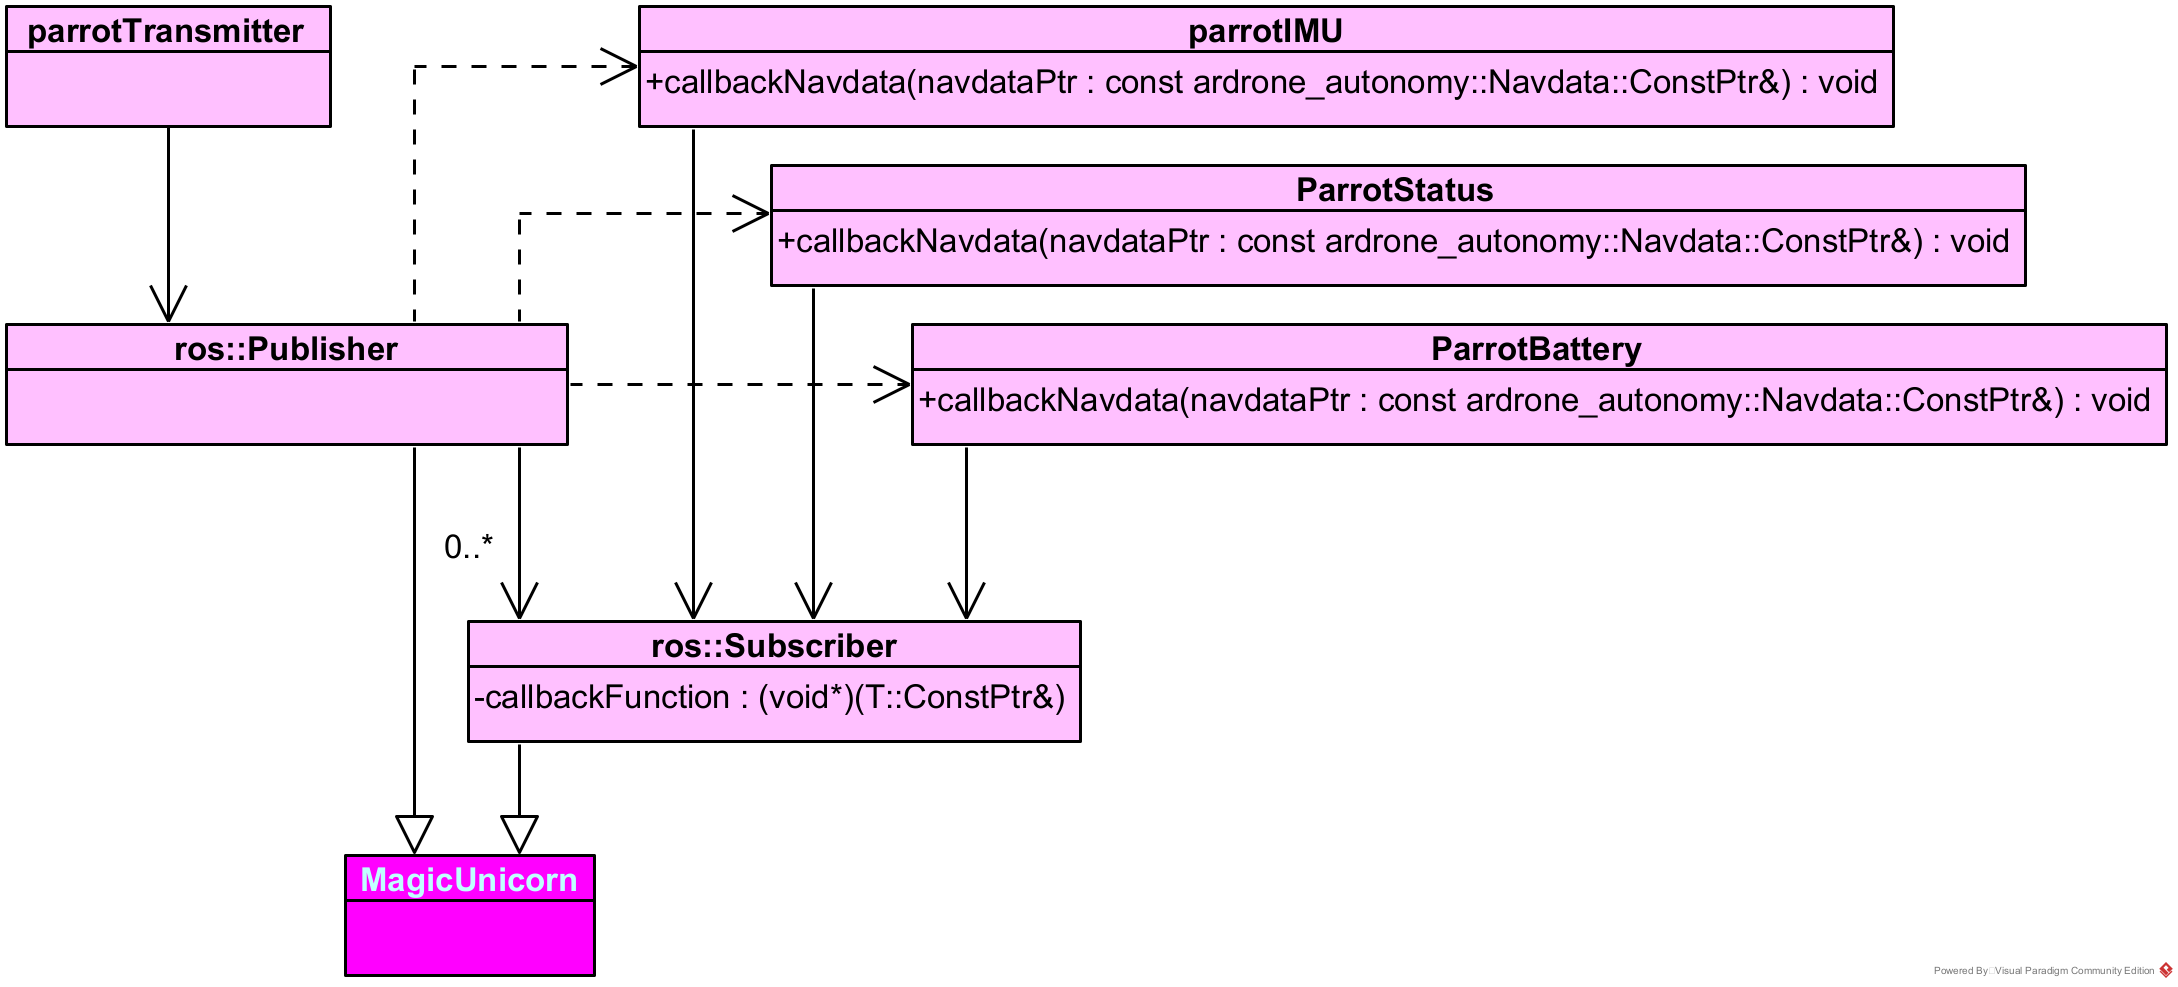
\includegraphics[width=15cm]{Pictures/Observer.png}}
\caption{Observer im Projekt}
\label{fig:Obs}
\end{center}

\vspace{0.25cm}
\refImgShort{fig:Obs} zeigt \missing\
\end{figure}



\newSec{Motivation}{4}
\missing[Ist halt Grundlage von ROS]


Die \ROS-\Pub\ und \Sub\ kommunizieren über \Topic[s] miteinander. 



\comp{ROSObserer1}


The  and the turtleteleopkey node are communicating with each other over a ROS Topic. 
turtleteleopkey is publishing the key strokes on a topic, while turtlesim subscribes to the same topic to receive the key strokes. 

\missing[evtl überarbeiten ;)]
Alles, was wir nicht verstanden haben (oder nicht genauer erörtern wollten) wird durch den Platzhalter \textcolor{pink}{\textit{MagicUnicorn}} veranschaulicht.
Ernsthaft, bei Nachfragen selbst mal den ROS-Jungel durchkämmen.